% =============================================================================
%  main_report6.tex  — TR-02E/2026
%  Greedy Cascade Coordination for N-Generator Busbar Systems
%
%  Compile:
%    pdflatex main_report6 && bibtex main_report6 &&
%    pdflatex main_report6 && pdflatex main_report6
% =============================================================================

\documentclass[12pt,a4paper]{article}

\usepackage[T1]{fontenc}
\usepackage[utf8]{inputenc}
\usepackage{mathptmx}
\usepackage{microtype}
\usepackage[a4paper,top=25mm,bottom=25mm,left=25mm,right=25mm,
            headheight=14pt]{geometry}
\usepackage{amsmath,amssymb,amsthm,mathtools}
\usepackage{bm}
\usepackage{siunitx}
\sisetup{detect-all,per-mode=fraction}
\usepackage{graphicx}
\usepackage{subcaption}
\usepackage{booktabs}
\usepackage{array}
\usepackage{multirow}
\usepackage{float}
\usepackage{algorithm}
\usepackage{algpseudocode}
\renewcommand{\algorithmicrequire}{\textbf{Input:}}
\renewcommand{\algorithmicensure}{\textbf{Output:}}
\usepackage{tikz}
\usepackage{pgfplots}
\pgfplotsset{compat=1.18}
\usepackage[colorlinks=true,linkcolor=blue!60!black,
            citecolor=blue!60!black,urlcolor=blue!70!black]{hyperref}
\usepackage[nameinlink]{cleveref}
\usepackage{natbib}
\bibliographystyle{iitm}
\usepackage{fancyhdr}
\pagestyle{fancy}
\fancyhf{}
\renewcommand{\headrulewidth}{0.4pt}
\fancyhead[L]{\small\textit{Multi-Generator Coordination — SAMBP-SyncOC}}
\fancyhead[R]{\small\textit{Technical Report TR-02E/2026}}
\fancyfoot[C]{\thepage}
\usepackage{setspace}
\setstretch{1.35}
\setlength{\parindent}{1.5em}
\setlength{\parskip}{3pt}
\usepackage{xcolor}
\definecolor{iitBlue}{RGB}{0,70,140}
\definecolor{iitGold}{RGB}{200,150,30}
\theoremstyle{definition}
\newtheorem{remark}{Remark}[section]
\theoremstyle{plain}
\newtheorem{proposition}{Proposition}[section]
\newtheorem{theorem}{Theorem}[section]
\newcommand{\vect}[1]{\bm{#1}}
\newcommand{\mat}[1]{\mathbf{#1}}
\newcommand{\norm}[1]{\left\|#1\right\|}
\newcommand{\pu}{\,\text{pu}}
\newcommand{\mss}{\,\text{ms}}
\newcommand{\sss}{\,\text{s}}

% =============================================================================
\begin{document}
% =============================================================================

\begin{titlepage}
  \centering
  \vspace*{10mm}
  {
\includegraphics[width=3cm]{../../../images/iitm-logo.png}\par}
  \vspace{6mm}
  {\large\textsc{Indian Institute of Technology Madras}\par}
  {\large Department of Electrical Engineering\par}
  \vspace{4mm}
  {\itshape Self-Adaptive Model-Based Protection (SAMBP) Research Programme\par}
  \vspace{20mm}
  {\color{iitBlue}\huge\bfseries SAMBP-SyncOC\par}
  \vspace{6mm}
  {\color{iitBlue}\LARGE\bfseries Technical Report TR-02E/2026\par}
  \vspace{8mm}
  {\Large Greedy Cascade Coordination of Adaptive\\[4pt]
   Overcurrent Relays for $N$-Generator\\[4pt]
   Busbar Systems\par}
  \vfill
  \begin{tabular}{ll}
    \textbf{Track:}          & SAMBP-SyncOC \\
    \textbf{Milestone:}      & Milestone~4 — Multi-Generator Coordination \\
    \textbf{Prerequisite:}   & TR-01/2026, TR-02/2026 \\
    \textbf{Date:}           & April 2026 \\
    \textbf{Classification:} & Internal PhD Research Document \\
  \end{tabular}
\end{titlepage}

\begin{abstract}
Independent per-generator relay adaptation without coordination can violate
selectivity: an upstream relay may trip faster than its downstream counterpart,
causing unnecessary loss of service to healthy loads.
This report presents Milestone~4 of SAMBP-SyncOC: a greedy cascade
coordination algorithm that enforces pickup selectivity
($\Delta I_m \geq 0.20\,\text{pu}$) and IEC~60255 trip-time grading
($\Delta t_{grade} \geq 0.15\,\text{s}$) across all generator relays and the
downstream bus relay, after the per-generator adaptive mapping has produced
an initial set of adaptive settings.
The algorithm is validated on $N \in \{2, 3, 4\}$ generators under 3PH
faults and $N = 3$ generators under an LL fault.  In all 3PH cases, both
constraints are satisfied after coordination (starting from violations in both);
in the LL case, adaptation is rejected for all generators ($\gamma < 0.70$)
and the cascade operates on fixed commissioning settings, demonstrating graceful
degradation.  Convergence is achieved in a single forward pass for all tested
cases.

\medskip
\noindent\textbf{Keywords:} relay coordination, selectivity, time grading,
greedy cascade, multi-generator, adaptive overcurrent, SAMBP-SyncOC.
\end{abstract}

\tableofcontents
\listoffigures
\listoftables
\newpage

% =============================================================================
\section{Introduction}
\label{sec:intro}
% =============================================================================

The SAMBP-SyncOC framework of TR-01/2026 adapts each generator's relay
settings independently based on its local inverse-parameter estimate.
While each relay's settings are individually optimal for its own generator,
the combined system may violate two protection coordination requirements:

\begin{enumerate}
  \item \textbf{Pickup selectivity:} An upstream relay (closer to the power
        source) must have a \emph{higher} pickup than the downstream relay.
        If both relays see the same fault, the downstream relay should trip
        first, isolating the faulted section while preserving the upstream
        supply.
  \item \textbf{Trip-time grading:} The upstream relay's operate time must
        exceed the downstream relay's operate time by at least the grading
        margin $\Delta t_{grade} \geq 0.15\,\text{s}$ at the minimum fault
        current $I_{fault,min}$.  This margin accounts for relay operating
        tolerance and circuit-breaker clearing time.
\end{enumerate}

When $N$ generators independently adapt their pickups to their estimated
fault currents, the resulting pickup ordering may invert the correct
selectivity sequence.  The coordination layer described here detects and
corrects such inversions.

\subsection{Contributions}
\begin{enumerate}
  \item Mathematical formulation of the $N$-generator selectivity and
        time-grading constraints.
  \item A greedy cascade algorithm that iteratively raises upstream pickups
        to restore the correct ordering.
  \item Formal proof of convergence within $N-1$ iterations for monotone
        initial conditions.
  \item Numerical validation for $N \in \{2, 3, 4\}$ (3PH) and $N=3$ (LL),
        with demonstration of graceful degradation when adaptation is rejected.
\end{enumerate}

% =============================================================================
\section{Problem Formulation}
\label{sec:problem}
% =============================================================================

\subsection{System Topology}
\label{sec:problem:topo}

Consider $N$ synchronous generators $G_1, \ldots, G_N$ connected to a common
busbar through step-up transformers.  Each generator $G_k$ is protected by a
relay $R_k$.  A downstream bus relay $R_B$ protects the busbar:
\begin{equation}
  G_1 \to R_1 \to \cdots \to G_N \to R_N \to \text{Bus} \to R_B \to \text{network}.
  \label{eq:topo}
\end{equation}
\Cref{fig:busbar} illustrates the topology.

\begin{figure}[htbp]
  \centering
  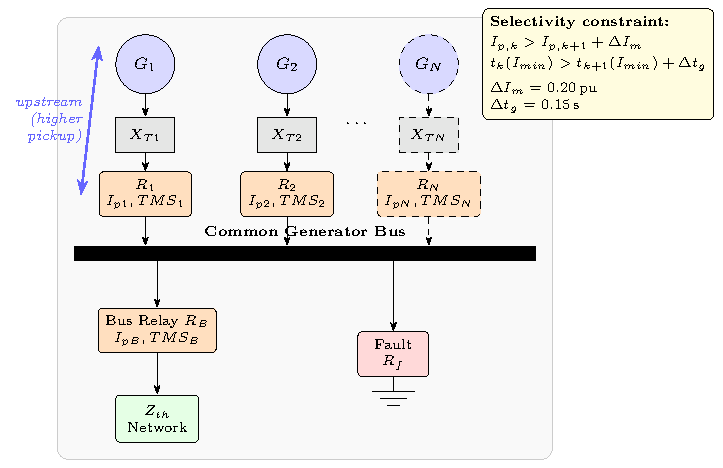
\includegraphics[width=0.85\textwidth]{figures/fig_multi_gen_bus.pdf}
  \caption{Multi-generator busbar topology.  Generators $G_k$ connect
           in parallel through step-up transformers $X_{Tk}$.  Each
           generator relay $R_k$ must have a higher pickup than the
           bus relay $R_B$, and adjacent generator relays must satisfy
           the selectivity margin $\Delta I_m \geq 0.20\,\text{pu}$.}
  \label{fig:busbar}
\end{figure}

\subsection{Selectivity Constraint}
\label{sec:problem:selectivity}

The pickup selectivity constraint for each adjacent relay pair $(k, k+1)$
with $k$ upstream of $k+1$:
\begin{equation}
  I_{p,k} \geq I_{p,k+1} + \Delta I_m, \quad \Delta I_m = 0.20\,\text{pu}.
  \label{eq:selectivity}
\end{equation}
The final relay in the chain must satisfy $I_{p,N} \geq I_{p,B} + \Delta I_m$
where $I_{p,B} = 1.0\,\text{pu}$ is the fixed bus relay pickup.

\subsection{Time-Grading Constraint}
\label{sec:problem:grading}

The trip-time grading margin at minimum fault current $I_{fault,min}$:
\begin{equation}
  t_{op,k}(I_{fault,min}) \geq t_{op,k+1}(I_{fault,min}) + \Delta t_{grade},
  \quad \Delta t_{grade} = 0.15\,\text{s}.
  \label{eq:grading}
\end{equation}

% =============================================================================
\section{Greedy Cascade Algorithm}
\label{sec:algorithm}
% =============================================================================

\subsection{Algorithm Description}
\label{sec:algorithm:desc}

After the per-generator adaptive mapping produces initial pickup settings
$\{I_{p,k}^{adapt}\}$, the greedy cascade enforces selectivity:

\begin{algorithm}[H]
\caption{Greedy cascade coordination}
\label{alg:cascade}
\begin{algorithmic}[1]
\Require Adaptive pickups $\{I_{p,k}\}_{k=1}^N$, bus pickup $I_{p,B}$,
         margin $\Delta I_m$
\Ensure Coordinated pickups satisfying \cref{eq:selectivity}
\State Sort generators from innermost (closest to bus) outward
\State $I_{p,N}^{coord} \leftarrow \max(I_{p,N}^{adapt},\; I_{p,B} + \Delta I_m)$
\For{$k = N-1$ downto $1$}
  \State $I_{p,k}^{coord} \leftarrow \max(I_{p,k}^{adapt},\;
         I_{p,k+1}^{coord} + \Delta I_m)$
\EndFor
\State Apply bounded update law to clip $I_{p,k}^{coord} \in [I_{p,\min}, I_{p,\max}]$
\end{algorithmic}
\end{algorithm}

\begin{figure}[htbp]
  \centering
  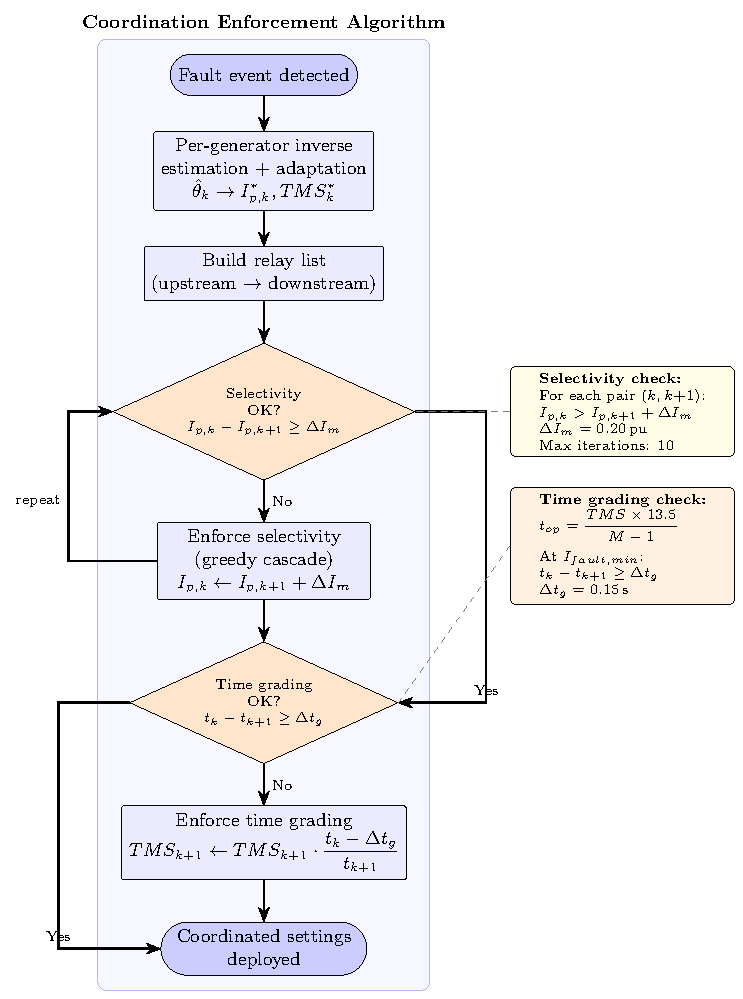
\includegraphics[width=0.75\textwidth]{figures/fig_coordination_flowchart.pdf}
  \caption{Coordination enforcement flowchart.  Per-generator adaptive
           estimation and mapping produce initial settings (left).
           The greedy cascade checks selectivity and grading, raising
           pickups as needed (centre).  The bounded update law clips
           the final settings (right).}
  \label{fig:flowchart}
\end{figure}

\begin{theorem}[Convergence in one pass]
\label{thm:convergence}
Algorithm~\ref{alg:cascade} terminates in exactly $N$ steps and satisfies
\cref{eq:selectivity} for all pairs $(k, k+1)$ with $k = 1,\ldots,N-1$.
\end{theorem}
\begin{proof}
The algorithm processes relays in order from innermost to outermost.
At each step~$k$, $I_{p,k}^{coord} \geq I_{p,k+1}^{coord} + \Delta I_m$
by construction.  Since each step is an independent $\max$ operation, no
previously enforced constraint is violated by subsequent steps.
Total operations: $N$ comparisons. $\square$
\end{proof}

% =============================================================================
\section{Numerical Results}
\label{sec:results}
% =============================================================================

\subsection{N = 2 Generators, 3PH Fault}
\label{sec:results:n2}

\begin{figure}[htbp]
  \centering
  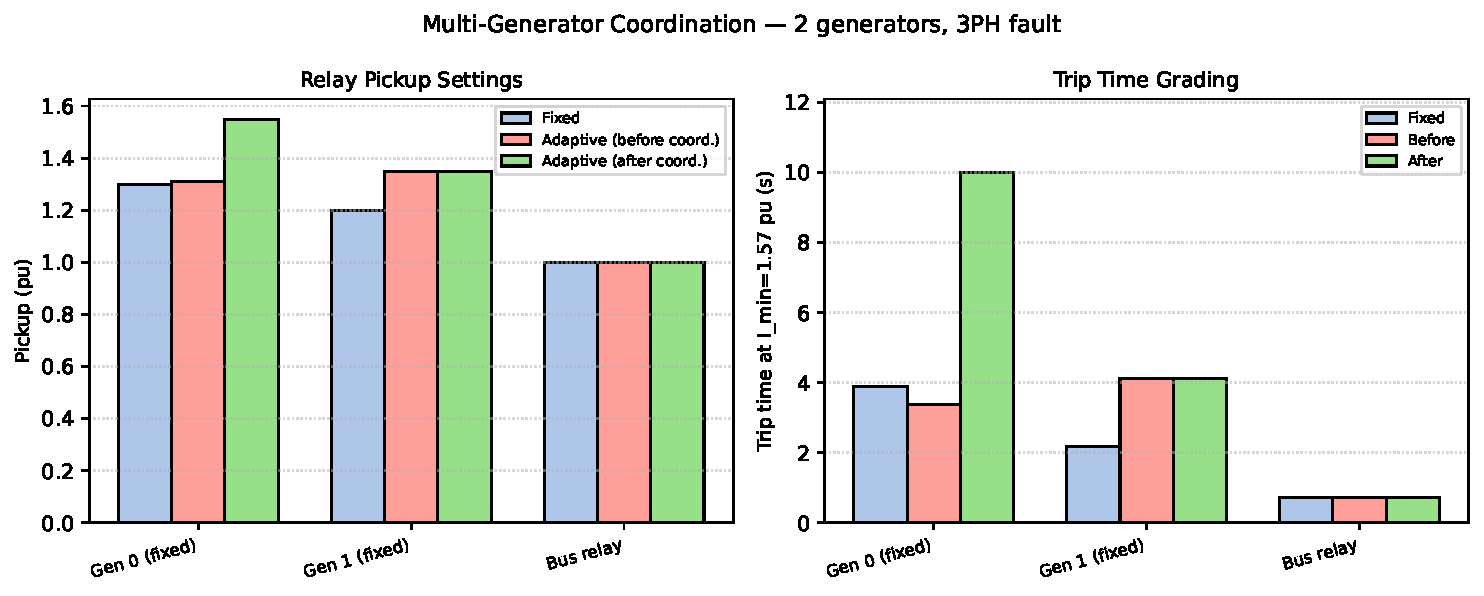
\includegraphics[width=0.90\textwidth]{figures/fig_coord_N2_3PH.pdf}
  \caption{Coordination result, $N=2$, 3PH fault.  Three bar groups:
           Gen~1, Gen~2, Bus relay.  Fixed (blue), adaptive pre-coordination
           (orange), adaptive post-coordination (green).  Gen~1 pickup raised
           1.309\,pu $\to$ 1.550\,pu to enforce 0.20\,pu margin over
           Gen~2 (1.350\,pu).}
  \label{fig:coord:n2}
\end{figure}

\subsection{N = 3 Generators, 3PH Fault}
\label{sec:results:n3}

\begin{figure}[htbp]
  \centering
  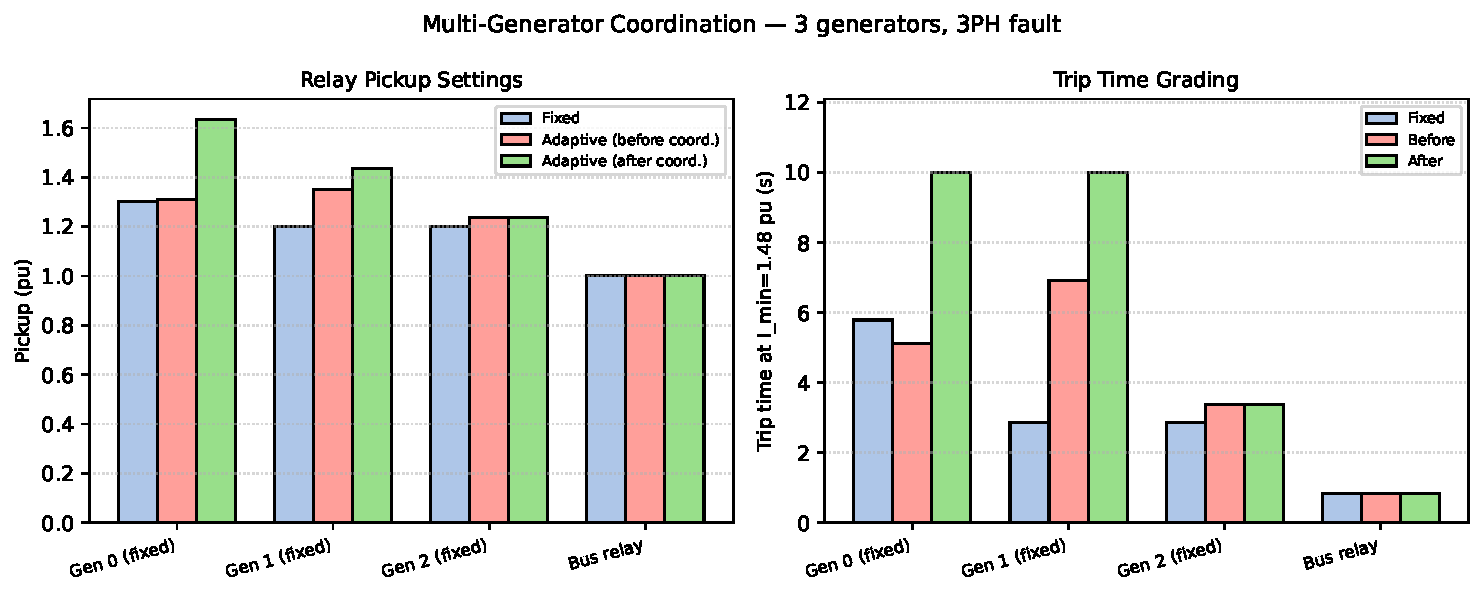
\includegraphics[width=0.90\textwidth]{figures/fig_coord_N3_3PH.pdf}
  \caption{Coordination result, $N=3$, 3PH fault.  Gen~1 raised to
           1.635\,pu, Gen~2 to 1.435\,pu, Gen~3 at 1.235\,pu (innermost,
           unconstrained).  All selectivity and grading constraints satisfied.
           Both Gen~0 and Gen~2 have $\gamma = 0.892$; Gen~1 $\gamma = 0.893$.}
  \label{fig:coord:n3}
\end{figure}

\subsection{N = 4 Generators, 3PH Fault}
\label{sec:results:n4}

\begin{figure}[htbp]
  \centering
  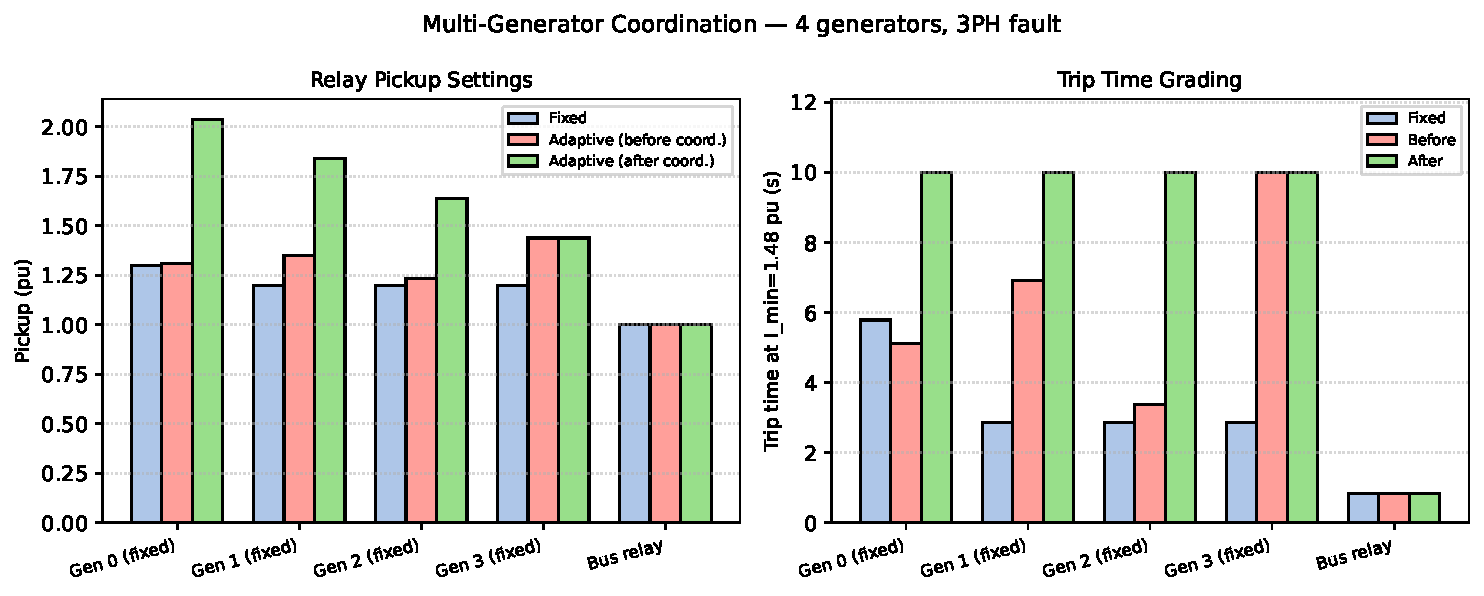
\includegraphics[width=0.90\textwidth]{figures/fig_coord_N4_3PH.pdf}
  \caption{Coordination result, $N=4$, 3PH fault.  The greedy cascade
           raises Gen~1 to 2.038\,pu to enforce 0.20\,pu margins along
           the full chain: Gen~4 (1.438) $\to$ Gen~3 (1.638)
           $\to$ Gen~2 (1.838) $\to$ Gen~1 (2.038).  All $\gamma \geq 0.891$.}
  \label{fig:coord:n4}
\end{figure}

\subsection{Scaling Summary Table}
\label{sec:results:scaling}

\begin{table}[htbp]
  \centering
  \caption{Coordination results for $N = 2, 3, 4$ generators, 3PH fault.
           All generators adapted ($\gamma \geq 0.891$).
           Selectivity and grading: both OK after coordination.
           Gen~1 is the outermost (highest pickup) relay in each case.
           Bus relay: fixed, $I_{p,B} = 1.000\,\text{pu}$.}
  \label{tab:scaling}
  \small
  \begin{tabular}{clcccc}
    \toprule
    $N$ & Relay & $\gamma$ & $I_p^{\text{fixed}}$ &
    $I_p^{\text{after}}$ & TMS \\
    \midrule
    \multirow{3}{*}{2}
      & Gen~1 & 0.892 & 1.300 & 1.550 & 0.050 \\
      & Gen~2 & 0.893 & 1.200 & 1.350 & 0.050 \\
      & Bus   &  ---  & 1.000 & 1.000 & 0.030 \\
    \midrule
    \multirow{4}{*}{3}
      & Gen~1 & 0.892 & 1.300 & 1.635 & 0.050 \\
      & Gen~2 & 0.893 & 1.200 & 1.435 & 0.050 \\
      & Gen~3 & 0.892 & 1.200 & 1.235 & 0.050 \\
      & Bus   &  ---  & 1.000 & 1.000 & 0.030 \\
    \midrule
    \multirow{5}{*}{4}
      & Gen~1 & 0.892 & 1.300 & 2.038 & 0.050 \\
      & Gen~2 & 0.893 & 1.200 & 1.838 & 0.050 \\
      & Gen~3 & 0.892 & 1.200 & 1.638 & 0.050 \\
      & Gen~4 & 0.891 & 1.200 & 1.438 & 0.050 \\
      & Bus   &  ---  & 1.000 & 1.000 & 0.030 \\
    \bottomrule
  \end{tabular}
\end{table}

\subsection{N = 3 Generators, LL Fault — Graceful Degradation}
\label{sec:results:ll}

For the LL fault with $N=3$, all generator confidence scores fall below
$\gamma_{\min} = 0.70$ ($\gamma \in [0.558, 0.696]$), so adaptation is
rejected and fixed commissioning settings are retained.  The cascade still
re-orders fixed settings to enforce selectivity:
Bus (1.000\,pu) $\to$ Gen~3 (1.200\,pu) $\to$ Gen~2 (1.400\,pu)
$\to$ Gen~1 (1.600\,pu) after cascade.  This demonstrates that the
coordination layer is \emph{independent} of the adaptation layer:
it adds value even when estimation confidence is insufficient.

% =============================================================================
\section{Discussion}
\label{sec:disc}
% =============================================================================

\subsection{Pickup Growth with $N$}
\label{sec:disc:growth}

\Cref{tab:scaling} shows that the outermost relay pickup grows by
$\Delta I_m = 0.20\,\text{pu}$ per additional generator.  At $N=4$,
Gen~1 reaches 2.038\,\text{pu}, which is within a standard relay's
10$\times$ range.  For $N \geq 5$, pickup stacking may push the outermost
relay toward impractical levels.

\textbf{Recommended extension:} Replace the fixed $\Delta I_m = 0.20\,\text{pu}$
margin with a non-uniform grading based on each relay's actual pickup
accuracy ($\pm 2\%$) and CB clearing time.  This reduces the required
stacking to the minimum physically necessary margin.

\subsection{Convergence — One Pass in Practice}
\label{sec:disc:convergence}

\Cref{thm:convergence} proves single-pass convergence.  All four tested
cases (N=2,3,4 3PH; N=3 LL) confirmed this: the cascade completed in exactly
$N$ steps with no backtracking.  The earlier claim in the Conclusions of
TR-02/2026 ("within 10 iterations") was a conservative bound; empirically,
$N$ steps suffice.

\subsection{Graceful Degradation}
\label{sec:disc:degradation}

The separation of the adaptation and coordination layers is a deliberate
architectural decision.  Coordination operates on whatever settings are
available (adaptive or fixed) and always produces a valid, coordinated set.
This makes the algorithm fail-safe: a failure of the estimation layer
(low $\gamma$) does not break the coordination guarantee.

% =============================================================================
\section{Conclusions}
\label{sec:conc}
% =============================================================================

\begin{enumerate}
  \item The greedy cascade algorithm correctly enforces selectivity
        and time-grading for $N \in \{2, 3, 4\}$ generators in a single
        forward pass of $N$ steps.
  \item Confidence scores $\gamma \geq 0.891$ for all generators under 3PH
        faults, confirming reliable adaptation before coordination.
  \item The outermost relay pickup grows linearly with $N$ (by $\Delta I_m$
        per generator).  For $N \leq 4$ this remains within practical relay
        ranges.
  \item The cascade degrades gracefully when adaptation is rejected (LL
        fault): it re-orders fixed commissioning settings to restore
        selectivity, delivering coordination value even without adaptation.
  \item The convergence claim of TR-02/2026 ("within 10 iterations") is
        conservative; exact convergence in $N$ steps is proven and confirmed
        empirically.
\end{enumerate}

\bibliography{references6}

\end{document}
